\subsubsection{postprocessing}
        Grundlegende Struktur des Postprocessing; beschreibt die Einbindung des 
        MotionBlurFilter in die JMonkeyEngine vorgaben\par
        \begin{figure}[htbp]
            \centering
            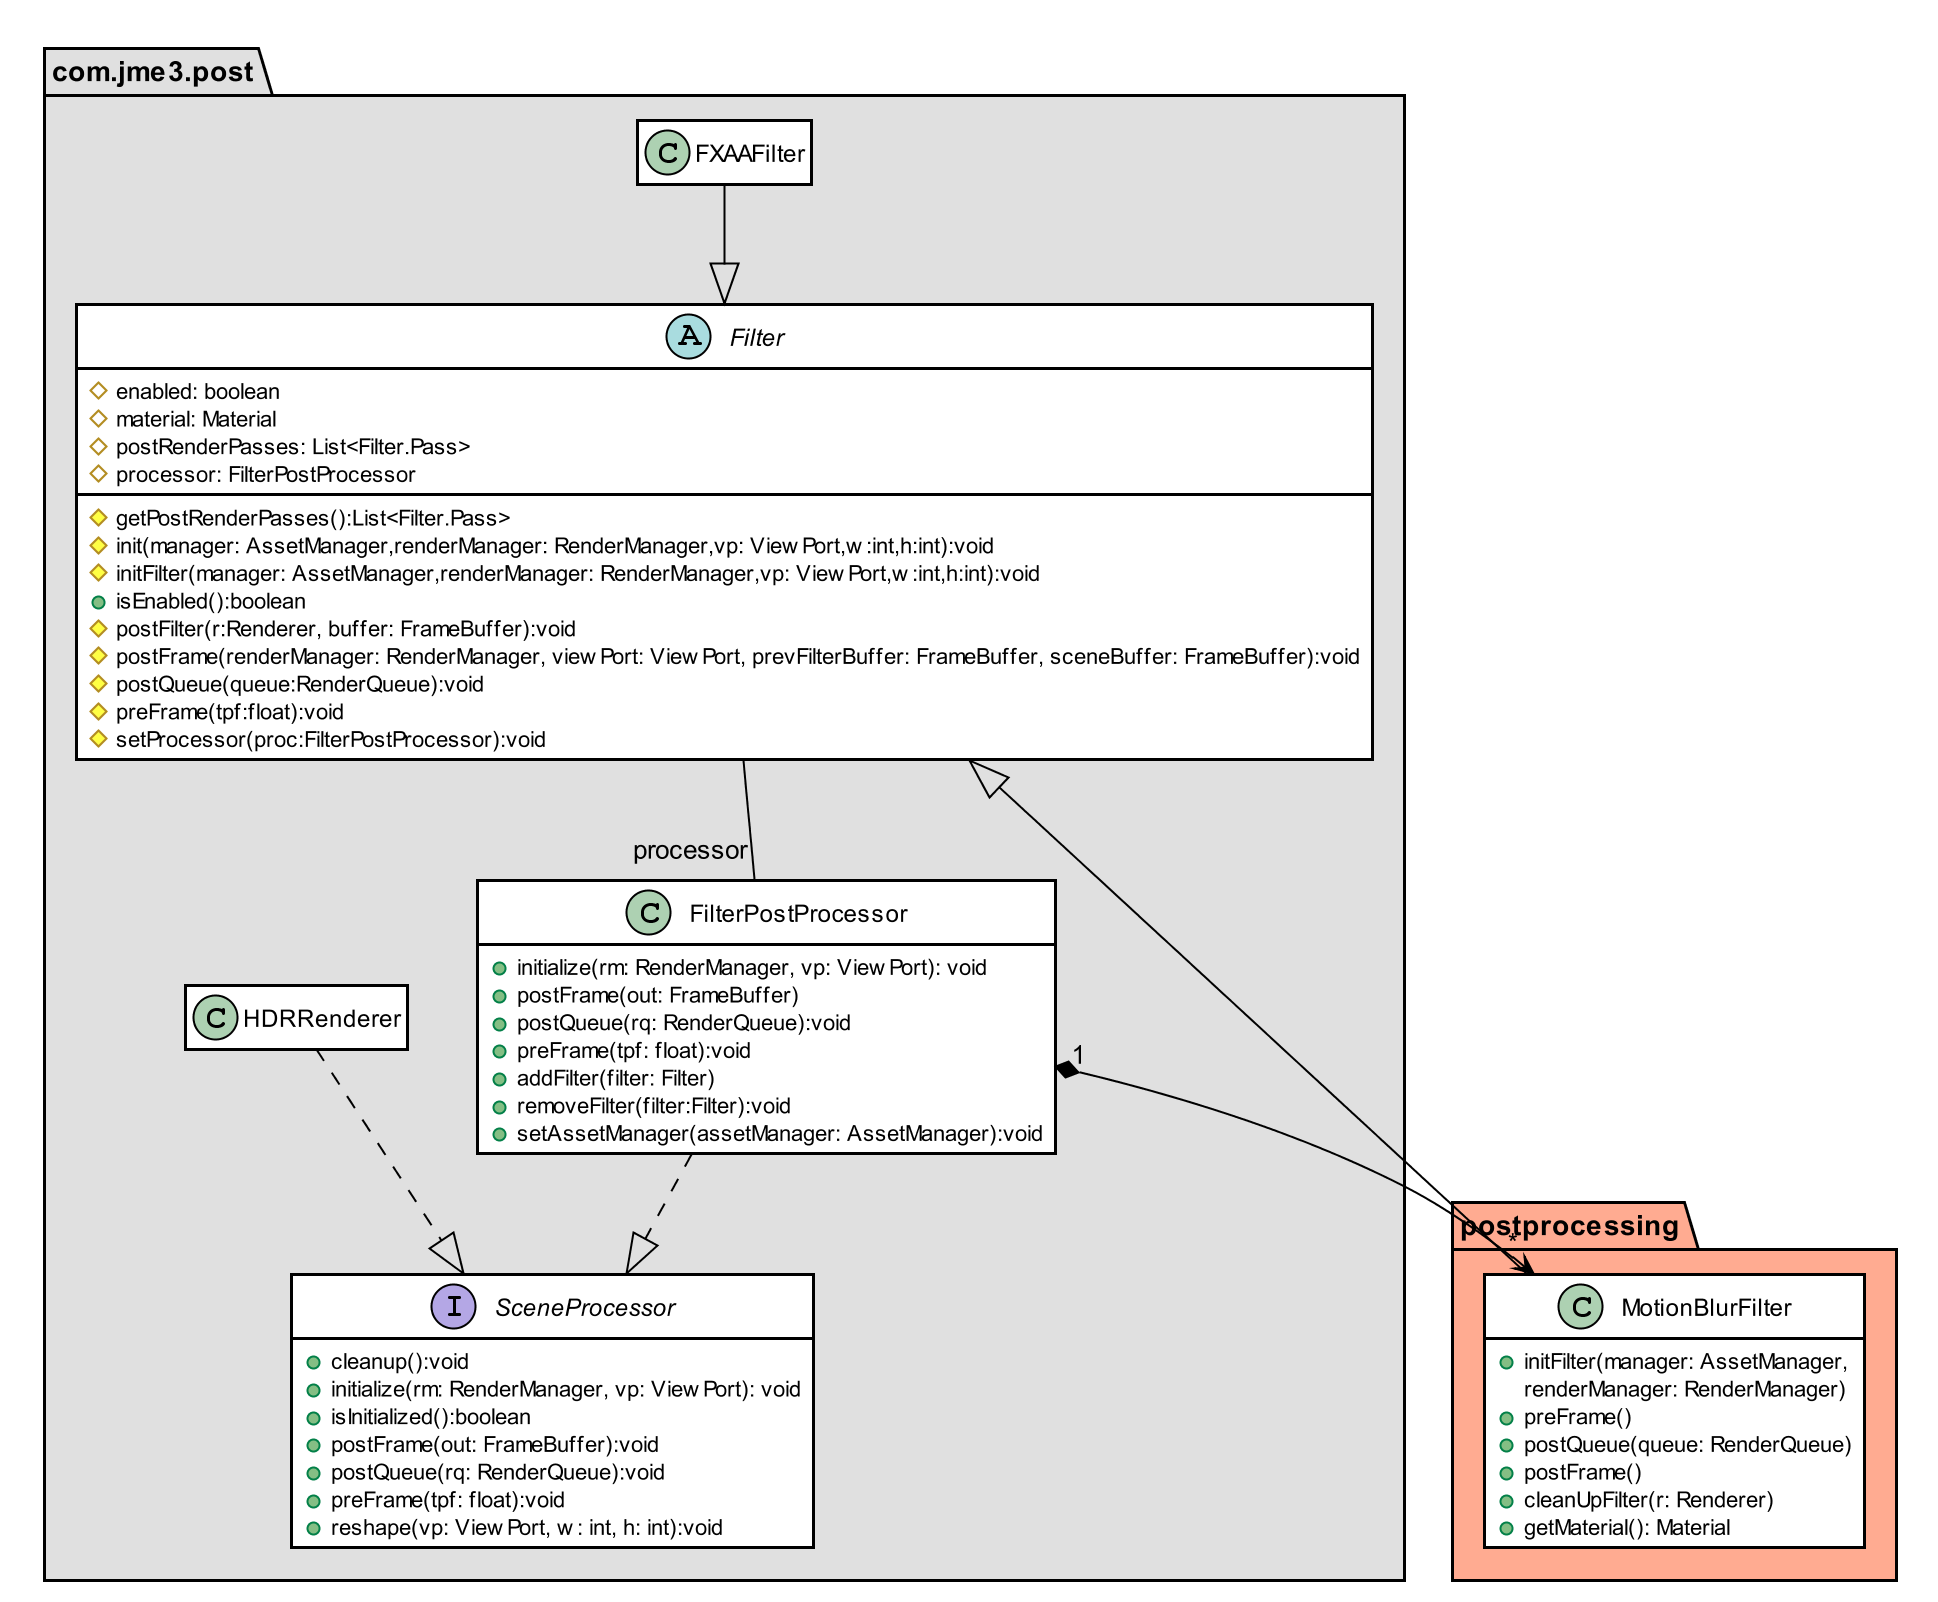
\includegraphics[width=1\linewidth]{InGameGrafik/Bilder/postprocessing.png}
            \caption{Klassendiagramm postprocessing}
        \end{figure}
            \paragraph{\underline{MotionBlurFilter}} \mbox{}\\
                    Visueller Effekt der Bewegungsunschärfe.\par
\pagebreak